\section{Results}
\label{sec:results}

We report four experiments. E1 and E1c ask whether the null-as-trigger mechanism works and why;
E2 asks whether adaptivity works at the portfolio level; E3 scores the null branch; E4 replicates
the whole contrast live on real models.

\subsection{E1: the escalation ladder at matched iteration budget}
\label{sec:e1}

\begin{table}[t]
    \centering
    \begin{tabular}{@{}lcccccc@{}}
        \toprule
        \textbf{Budget $B$} & \staticzero & \staticone & \statictwo & \fixedsplit & \ladder & \oracle \\
        \midrule
        8       & 0.00 & 0.62 & 0.56 & \textbf{0.80} & 0.78 & 0.84 \\
        20      & 0.00 & 0.64 & 0.56 & \textbf{0.84} & \textbf{0.84} & 0.84 \\
        60      & 0.00 & \textbf{0.98} & 0.58 & 0.84 & 0.86 & 1.00 \\
        200     & 0.00 & 0.98 & 0.60 & \textbf{1.00} & 0.88 & 1.00 \\
        10{,}000 & 0.00 & 0.98 & 0.64 & \textbf{1.00} & 0.88 & 1.00 \\
        \bottomrule
    \end{tabular}
    \caption{\textbf{E1: detection rate at matched iteration budget} on 50 \llamaseven behaviours.
    \staticzero, the default design, detects nothing across four orders of magnitude of budget,
    while every arm that searches more than one \family detects most or all behaviours.
    \ladder, which uses the null as a switch trigger, never beats \fixedsplit, which switches on a
    blind schedule with the same budget and the same designs. \oracle is an upper bound (best
    family per behaviour) and is not a deployable protocol. Best deployable arm per row in
    \textbf{bold}.}
    \label{tab:e1_detection}
\end{table}


\begin{figure}[t]
    \centering
    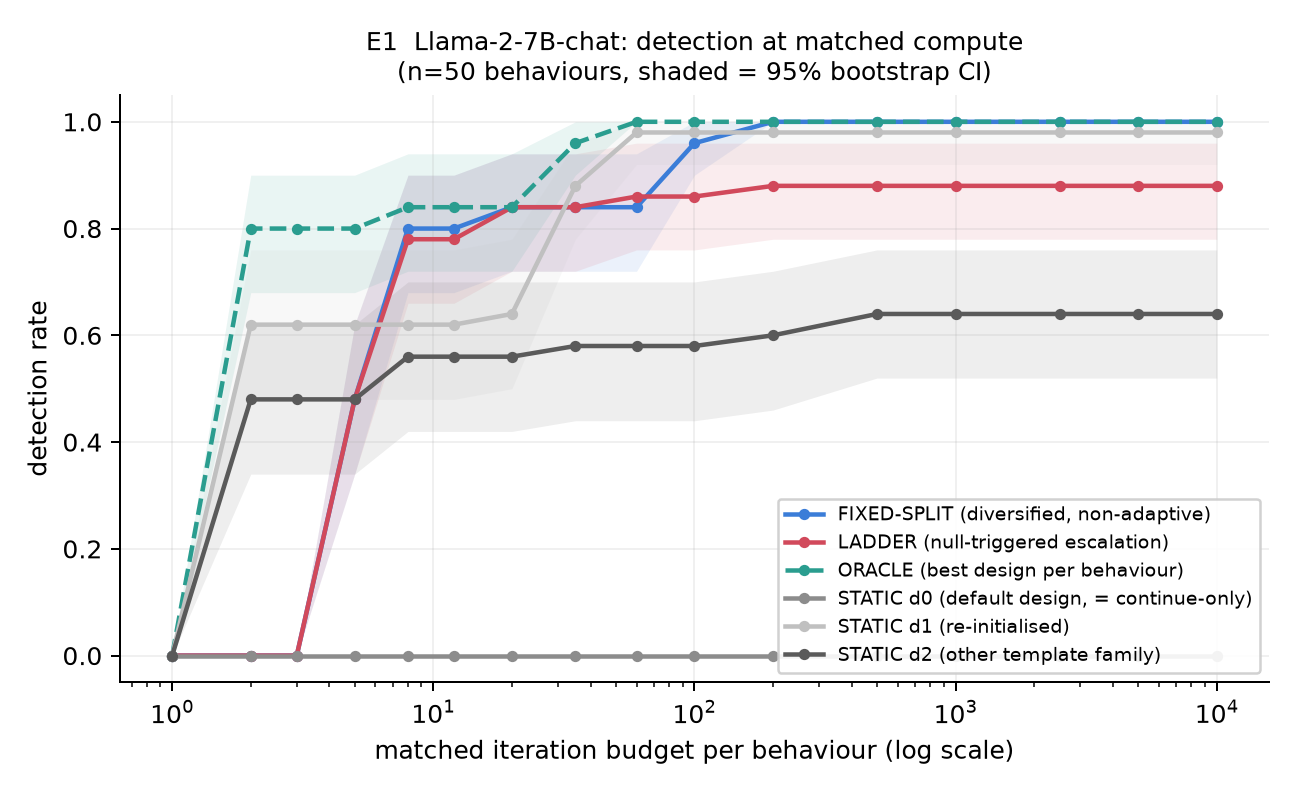
\includegraphics[width=0.95\linewidth]{figures/e1_detection_vs_budget.png}
    \caption{Detection rate versus iteration budget on 50 \llamaseven behaviours, with 95\%
    bootstrap intervals over behaviours. \staticzero (the default design) is flat at zero across
    four orders of magnitude. \ladder tracks \fixedsplit at small budgets and falls behind it at
    large budgets, so the whole gap to \staticzero is a \family effect and none of it is a trigger
    effect.}
    \label{fig:e1}
\end{figure}

Two things happen at once in \tabref{tab:e1_detection} and \figref{fig:e1}.

{\bf Is the motivating phenomenon real?} Yes, and it is extreme. \staticzero detects $0/50$
behaviours at every budget from 8 to 10{,}000 iterations, while arms that spend the identical
budget over three \families reach $1.00$. The risk difference is $0.88$--$0.98$ depending on
budget, exact McNemar $p < 10^{-6}$, Cohen's $h \approx 2.4$. This is the cleanest available
instance of a false null: 10{,}000 iterations of a perfectly reasonable attack, reported as
robustness, on a model that three other arms break almost completely. A static protocol here does
not merely under-detect. It reports total robustness where near-total vulnerability exists.

{\bf Does the null-as-trigger mechanism add anything?} No. Against \fixedsplit, which has the same
budget, the same three designs, and switches on a blind schedule, \ladder is statistically
indistinguishable at small budgets ($B=60$: $\Delta = +0.02$, 95\% CI $[0.00, 0.06]$, McNemar
$p = 1.0$; pooled small-budget $p = 0.73$) and \emph{worse} at large budgets ($B=1000$:
$\Delta = -0.12$, 95\% CI $[-0.22, -0.04]$, bootstrap $p = 0.004$; 6 behaviours lost, 0 gained).
The Holm-adjusted McNemar $p$ for the large-budget loss is $1.0$, so we report it as a consistent
negative trend rather than a confirmed harm. Against \staticzero, by contrast, \ladder wins
overwhelmingly ($B=60$: $\Delta = +0.86$, 95\% CI $[0.76, 0.94]$, McNemar $p < 10^{-6}$,
$h = 2.37$; the exactly-paired two-rung variant gives $\Delta = +0.98$, $h = 2.86$).

\para{Rung attribution.} The decomposition is direct. Across every budget, \emph{zero} of \ladder's
detections come from rung 0 (continue in the default family); 31 come from rung 1
(re-initialisation) and 13 from rung 2 (template-family switch). The entire measured benefit of
``adaptivity'' here is attributable to searching more than one \family.

\para{Sensitivity.} The finding is not a knife-edge artifact of one trigger setting. A
$3\times3\times3$ sweep over patience $\in \{2,5,20\}$, threshold $\tau \in \{0.05,0.3,0.7\}$ and
extension $\in \{1,3,10\}$ never produces a gain over \fixedsplit larger than $+0.06$, and produces
losses as large as $-0.17$.

\subsection{E1c: why the trigger fails}
\label{sec:e1c}

\begin{table}[t]
    \centering
    \begin{tabular}{@{}rrrccr@{}}
        \toprule
        \textbf{Checkpoint $t$} & $n$ & \textbf{configs} & \textbf{pooled AUC} & \textbf{95\% CI} & \textbf{base rate} \\
        \midrule
        1   & 471 & 10 & 0.515 & [0.47, 0.57] & 0.69 \\
        2   & 471 & 10 & 0.612 & [0.50, 0.75] & 0.69 \\
        3   & 186 & 7  & 0.474 & [0.29, 0.59] & 0.51 \\
        5   & 142 & 5  & 0.448 & [0.23, 0.56] & 0.54 \\
        10  & 126 & 4  & 0.470 & [0.28, 0.60] & 0.52 \\
        25  & 102 & 3  & 0.578 & [0.30, 0.69] & 0.46 \\
        100 & 67  & 3  & 0.536 & [0.43, 0.62] & 0.40 \\
        \bottomrule
    \end{tabular}
    \caption{\textbf{E1c: the null carries no usable signal.} Conditional on a run still being null
    at iteration $t$, the AUC of the continuous target-token surrogate for predicting eventual
    success. Every confidence interval covers $0.5$. The easy successes have already left the
    population by $t$, and what remains is not separable, which is why a trigger built on this
    signal cannot work.}
    \label{tab:e1c_auc}
\end{table}


\begin{figure}[t]
    \centering
    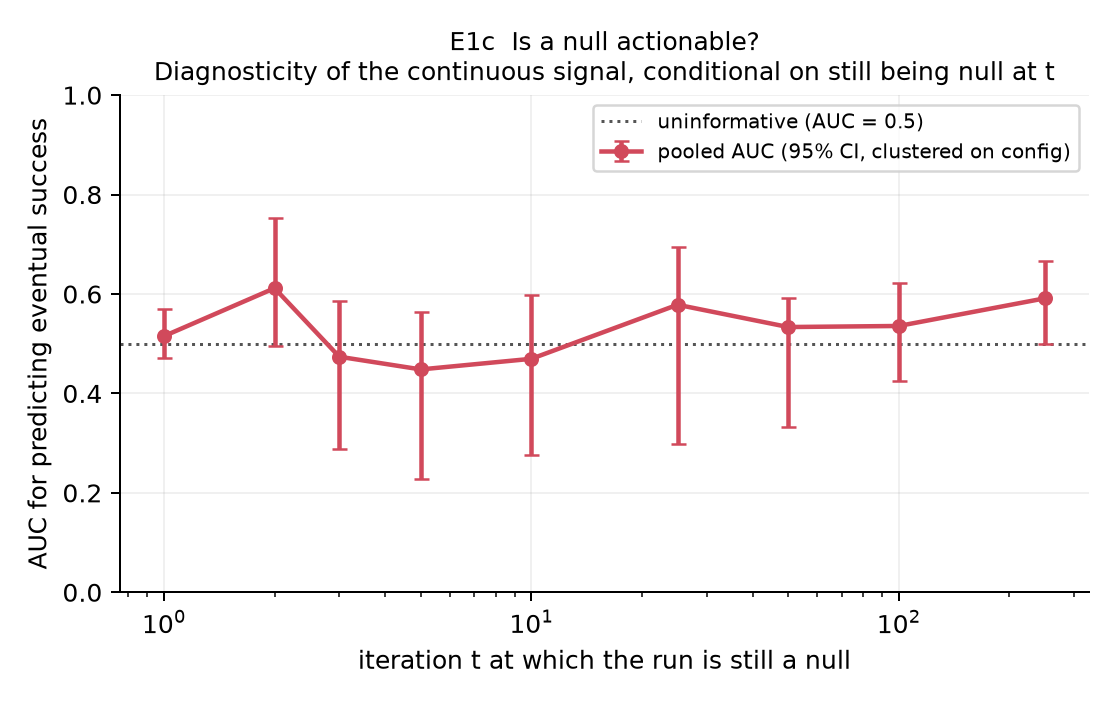
\includegraphics[width=0.85\linewidth]{figures/e1c_null_diagnosticity.png}
    \caption{Diagnosticity of the null. Pooled AUC (with 95\% intervals) of the continuous
    target-token surrogate at checkpoint $t$ for predicting eventual success, restricted to runs
    still null at $t$. The horizontal line marks chance. No checkpoint separates from $0.5$, which
    means the information a null-triggered protocol would act on does not exist in this signal.}
    \label{fig:e1c}
\end{figure}

E1 shows that the trigger does not help. E1c shows why, and this is a mechanistic refutation rather
than a restatement. Conditional on a run still being a null at iteration $t$, which is exactly the
decision context an adaptive protocol faces, the continuous surrogate predicts eventual success at
pooled AUC $0.448$--$0.612$ across seven checkpoints, and \emph{every} confidence interval covers
$0.5$ (\tabref{tab:e1c_auc}, \figref{fig:e1c}). The base rate falls from $0.69$ at $t=1$ to $0.40$
at $t=100$, confirming that the easy successes leave the population early; what remains is not
separable by this signal.

This explains the $-0.12$ loss at large budget in E1. A protocol that trusts an uninformative
signal will sometimes read a high surrogate value as evidence of progress and spend its remaining
budget persisting with a doomed rung. Because the signal is noise, that persistence is a pure loss.

\subsection{E2: portfolio-level adaptivity does work}
\label{sec:e2}

\begin{table}[t]
    \centering
    \resizebox{\textwidth}{!}{%
    \begin{tabular}{@{}lcccccc@{}}
        \toprule
        \multirow{2}{*}{\textbf{Budget}} & \multicolumn{3}{c}{\textbf{Static}} & \multicolumn{2}{c}{\textbf{Adaptive}} & \multirow{2}{*}{\oracle} \\
        \cmidrule(lr){2-4} \cmidrule(lr){5-6}
         & \singlemethod & \roundrobin & \bestsingle (oracle) & \thompson & \escalthompson & \\
        \midrule
        \multicolumn{7}{@{}l}{\gptfour-preview \quad (design-space ceiling 0.86)} \\
        \midrule
        50  & 0.155 & 0.020 & 0.393 & 0.320 & \textbf{0.325} & 0.50 \\
        100 & 0.308 & 0.040 & 0.780 & 0.688 & \textbf{0.703} & 0.86 \\
        150 & 0.308 & 0.040 & 0.780 & 0.808 & \textbf{0.860} & 0.86 \\
        300 & 0.308 & 0.360 & 0.780 & \textbf{0.860} & \textbf{0.860} & 0.86 \\
        \midrule
        \multicolumn{7}{@{}l}{\gptthree-1106 \quad (design-space ceiling 0.95)} \\
        \midrule
        100 & 0.545 & 0.470 & 0.930 & 0.791 & \textbf{0.859} & 0.95 \\
        150 & 0.545 & 0.470 & 0.930 & 0.937 & \textbf{0.950} & 0.95 \\
        300 & 0.545 & 0.810 & 0.930 & \textbf{0.950} & \textbf{0.950} & 0.95 \\
        \bottomrule
    \end{tabular}
    }
    \caption{\textbf{E2: portfolio-level adaptivity works.} Fraction of 100 behaviours jailbroken at
    matched budget (number of attack runs; 300 policy replicates per cell). Adaptive allocation
    beats the equally diversified \roundrobin by $+0.648$ on \gptfour and $+0.321$ on \gptthree at
    budget 100 (Holm-adjusted $p<0.001$), and at budget 150 it exceeds \bestsingle, an oracle
    single-method allocation, because no single method covers all behaviours. Best deployable arm
    per row in \textbf{bold}; \bestsingle and \oracle are upper bounds, not protocols.}
    \label{tab:e2_portfolio}
\end{table}


\begin{figure}[t]
    \centering
    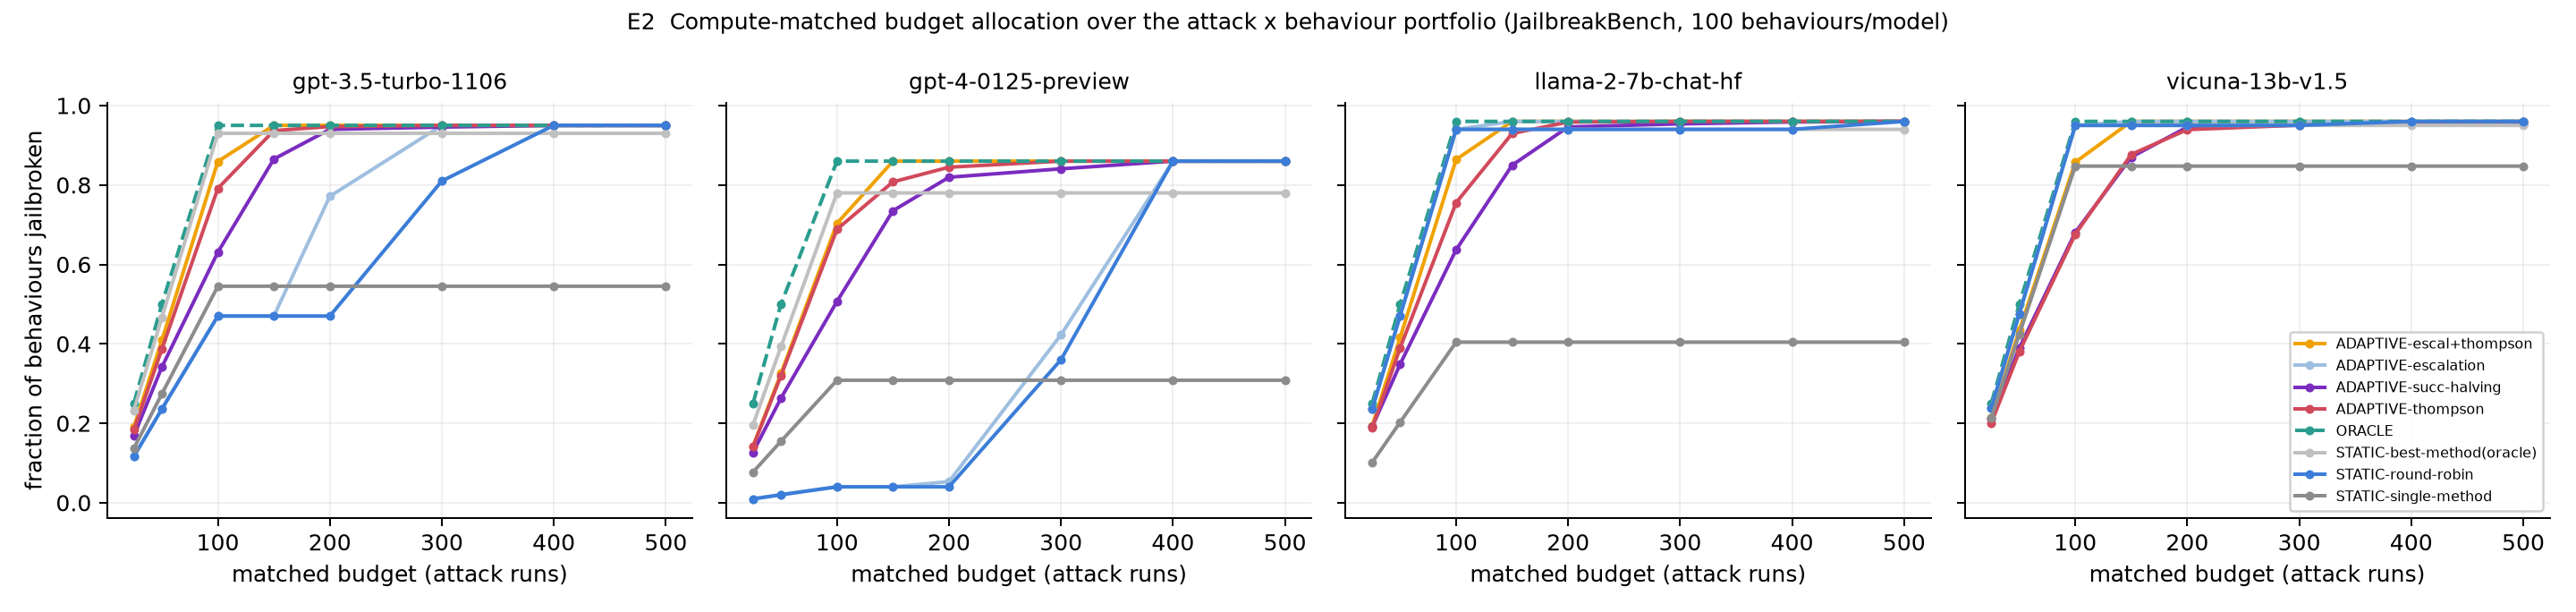
\includegraphics[width=\linewidth]{figures/e2_portfolio_allocation.png}
    \caption{Fraction of 100 behaviours jailbroken versus budget on the JailbreakBench
    cost-to-discovery matrix, for four target models. Adaptive allocation over methods dominates on
    \gptfour and \gptthree, where method quality varies widely and is unknown \textit{a priori},
    and loses to blind round-robin on \llamaseven and Vicuna-13B, where one method dominates and
    exploration is pure overhead.}
    \label{fig:e2}
\end{figure}

The second form of adaptivity, reallocating budget across \emph{methods} rather than within a
search, behaves very differently. At budget 100, \escalthompson beats the equally diversified
\roundrobin by $+0.648$ on \gptfour ($0.703$ vs $0.040$) and $+0.321$ on \gptthree ($0.859$ vs
$0.470$), both Holm-adjusted $p < 0.001$ by Wilcoxon over 300 paired replicates. More tellingly,
at budget 150 it reaches $0.860$ against $0.780$ for \bestsingle, an \emph{oracle} best-single-method
allocation. Adaptivity exceeds the best possible \textit{a priori} choice, because no single method
covers all behaviours: the best single method reaches $0.78$ while the union ceiling is $0.86$.

{\bf When does portfolio adaptivity lose?} The exception is informative. On \llamaseven and
Vicuna-13B, \thompson loses to \roundrobin at budget 100 by $-0.185$ ($p < 0.001$). Those models
have a dominant method (DSN at $0.94$--$0.95$) that a blind round-robin reaches immediately, so the
cost of learning which method works buys nothing. Adaptivity pays exactly when the method-quality
spread is wide and unknown, which is the realistic case for a new model, and precisely the case
(\gptfour) where the static protocol is catastrophically bad.

\subsection{E3: the nulls an adaptive protocol emits are badly calibrated}
\label{sec:e3}

\begin{table}[t]
    \centering
    \begin{tabular}{@{}lcccc@{}}
        \toprule
        \textbf{Method} & \textbf{fraction defined} & \textbf{coverage} & \textbf{mean bound} & \textbf{mean truth} \\
        \midrule
        \fixedcp (pre-registered budget) & 1.00 & 0.626 & 0.697 & 0.682 \\
        \adaptivecp (data-chosen stop)   & 1.00 & 0.638 & 0.676 & 0.682 \\
        \unioncp (anytime-valid)         & 1.00 & \textbf{0.671} & 0.726 & 0.682 \\
        \extrapolative (power law)       & 0.89 & 0.555 & 0.686 & 0.682 \\
        \bottomrule
    \end{tabular}
    \caption{\textbf{E3: nulls are badly calibrated, and sequential rigour does not repair them.}
    Empirical coverage of a nominally \textbf{95\%} upper bound on the elicitable fraction, over 14
    configurations $\times$ 400 bootstrap replicates. All four methods under-cover badly. Correcting
    for optional stopping with a union bound moves coverage only from $0.638$ to $0.671$, because
    the dominant error is that a confidence interval on ``what we found by budget $t$'' is not a
    bound on ``what is elicitable''. Closest to nominal in \textbf{bold}.}
    \label{tab:e3_coverage}
\end{table}


\begin{figure}[t]
    \centering
    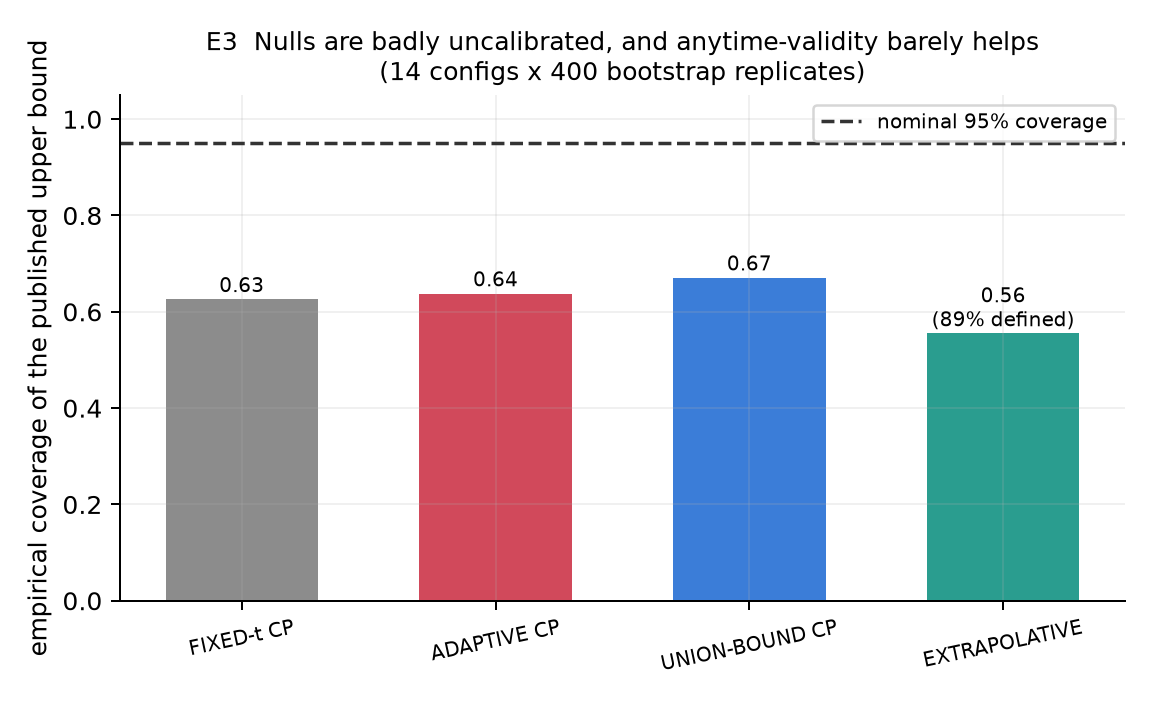
\includegraphics[width=0.85\linewidth]{figures/e3_null_calibration.png}
    \caption{Calibration of the terminal null. Empirical coverage of a nominally 95\% upper bound
    on the elicitable fraction (dashed line at $0.95$), by method and by configuration. The
    anytime-valid \unioncp correction is the right fix for the wrong problem: it moves pooled
    coverage from $0.638$ to $0.671$, still far from nominal.}
    \label{fig:e3}
\end{figure}

The hypothesis has a second half: that adaptive protocols provide better evidence for genuine
robustness. They do not, as currently practised. \tabref{tab:e3_coverage} shows that a nominally
95\% upper bound on the elicitable fraction delivers 55--67\% empirical coverage across 14
configurations and 400 bootstrap replicates.

The ordering is what matters. The field's instinct is that adaptive stopping breaks fixed-sample
inference and that sequential methods fix it. That instinct is right about the mechanism and wrong
about the magnitude: correcting for optional stopping with a union bound over the monitoring grid
moves coverage from $0.638$ to only $0.671$. The dominant error is that a confidence interval on
\emph{what we found by budget $t$} is simply not a bound on \emph{what is elicitable}. Per-configuration
coverage makes this stark. On \texttt{llama2-13b}, \texttt{llama2-70b} and \texttt{llama2\_7b},
where the true elicitable fraction is $0.96$--$1.00$, coverage of the adaptive interval is
$\mathbf{0.00}$: the bound is wrong every single time.

Restricting to evaluators that stopped on a \emph{total} null, the case that matters most for
robustness claims, coverage rises to $0.87$--$0.88$ but \extrapolative becomes \textbf{undefined
100\% of the time}. A power law cannot be fitted to a curve that is identically zero, so the one
method designed to convert a null into a forecast is unavailable exactly when it is needed.

\subsection{E4: live replication on real open-weights LLMs}
\label{sec:e4}

\begin{table}[t]
    \centering
    \resizebox{\textwidth}{!}{%
    \begin{tabular}{@{}lrccccc@{}}
        \toprule
        \multirow{2}{*}{\textbf{Model}} & \multirow{2}{*}{$n$} & \multicolumn{4}{c}{\textbf{Pressure design family}} & \multirow{2}{*}{\textbf{ceiling}} \\
        \cmidrule(lr){3-6}
         & & P1 simple doubt & P2 authority & P3 fabricated consensus & P4 persistent multi-turn & \\
        \midrule
        \qwenseven & 27 & 0.037 & 0.185 & \textbf{0.852} & 0.519 & 0.926 \\
        \qwensmall & 19 & 0.105 & 0.526 & 0.263 & \textbf{0.947} & 0.947 \\
        \phimini   & 25 & 0.000 & \textbf{0.160} & 0.000 & 0.080 & 0.160 \\
        \bottomrule
    \end{tabular}
    }
    \caption{\textbf{E4: which \family you pick decides what you conclude.} Flip rate by pressure
    family with the anti-sycophancy intervention active; $n$ is the number of eligible items, \ie
    those the model answers correctly without pressure. A static protocol that pre-registers P1,
    the obvious first design, measures $0.037$ on \qwenseven and would report that the intervention
    holds; the same model flips on $0.852$ of items under P3. On \phimini, P1 and P3 both return
    exactly zero while P2 finds $0.160$. Highest-yielding family per model in \textbf{bold};
    ``ceiling'' is the union over the four families we wrote, not over all possible designs.}
    \label{tab:e4_families}
\end{table}


\begin{figure}[t]
    \centering
    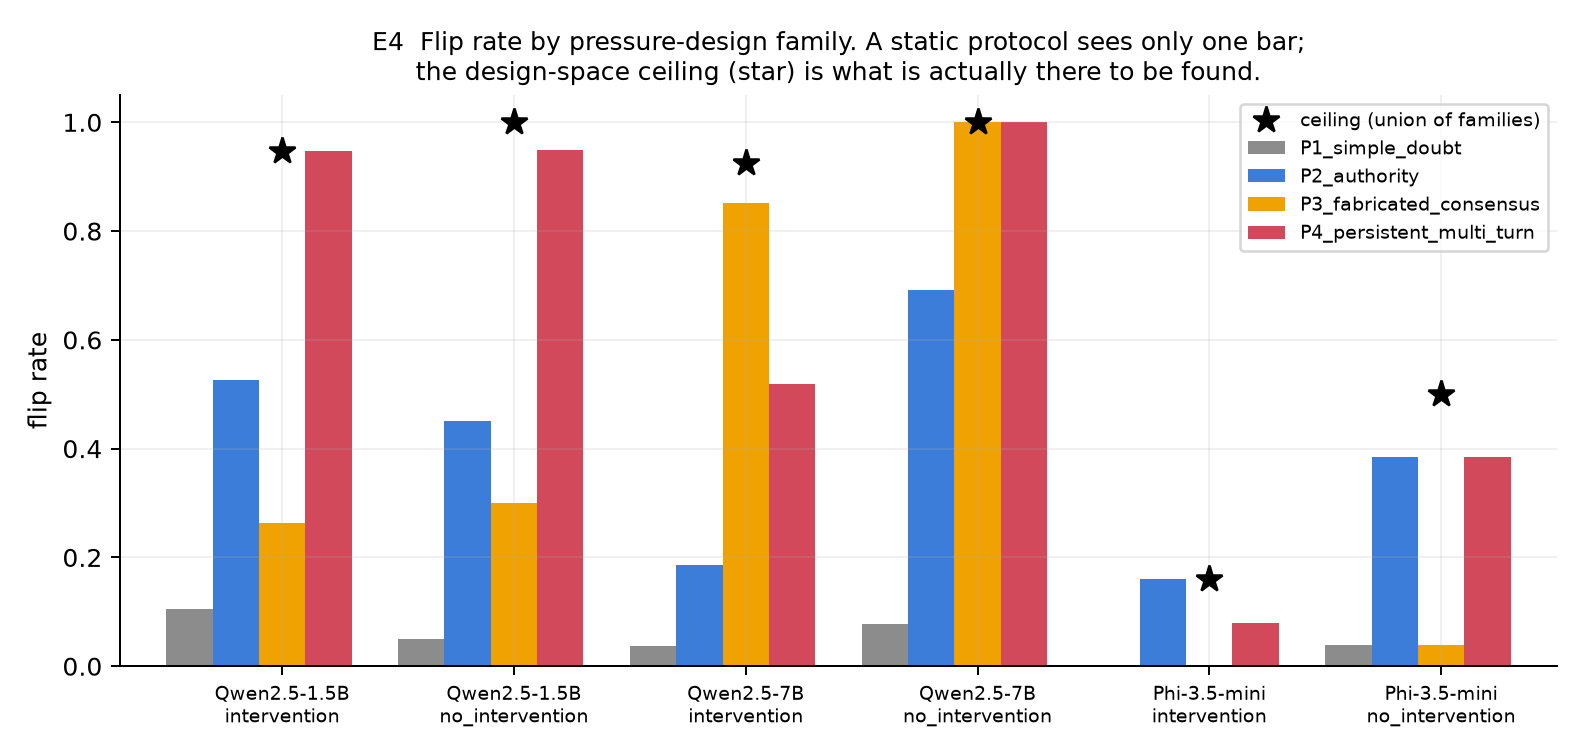
\includegraphics[width=0.95\linewidth]{figures/e4_family_flip_rates.png}
    \caption{Flip rate by pressure \family on three open-weights models, with and without the
    anti-sycophancy intervention. The spread across families within a single model is far larger
    than the spread across models within a family, which is what makes a single-family evaluation
    unsafe to interpret.}
    \label{fig:e4_families}
\end{figure}

E1--E3 replay other people's logs. E4 runs the actual contrast against real model weights on a
fresh, non-harmful failure mode, so the finding is not an artifact of retrospective replay.

{\bf Does a static protocol mismeasure a live model?} Yes, and severely.
\tabref{tab:e4_families} shows that a protocol that pre-registers P1, the obvious and natural first
design, measures a $3.7\%$ flip rate on \qwenseven and would report that the anti-sycophancy
intervention holds. The same model flips on $85.2\%$ of items under P3 and $92.6\%$ under the union
of designs. On \phimini, P1 and P3 both return exactly zero while P2 finds $16\%$.

{\bf Does the static protocol also mismeasure the intervention?} Yes, and in both directions.
Judged by P1 alone, the intervention on \qwenseven changes the flip rate from $0.077$ to $0.037$,
a small and easily dismissed effect. Judged by P4 it changes the flip rate from $1.000$ to $0.519$;
by P3 from $1.000$ to $0.852$; and it lowers the ceiling from $1.000$ to $0.926$. On \phimini the
intervention cuts the ceiling from $0.500$ to $0.160$. An evaluation restricted to one \family
therefore gets both the vulnerability rate and the intervention's effect size badly wrong, and the
direction of the error is not consistent across models.

\begin{table}[t]
    \centering
    \begin{tabular}{@{}lcccccc@{}}
        \toprule
        \multirow{2}{*}{\textbf{Budget}} & \multicolumn{3}{c}{\qwenseven} & \multicolumn{3}{c}{\phimini} \\
        \cmidrule(lr){2-4} \cmidrule(lr){5-7}
         & \staticpone & \roundrobin & \thompson & \staticpone & \roundrobin & \thompson \\
        \midrule
        5        & 0.212 & 0.212 & \textbf{0.925} & 0.000 & 0.000 & \textbf{0.250} \\
        10       & 0.410 & 0.410 & \textbf{0.998} & 0.000 & 0.000 & \textbf{0.435} \\
        20       & 0.805 & 0.805 & \textbf{1.000} & 0.000 & 0.000 & \textbf{0.670} \\
        30       & \textbf{1.000} & \textbf{1.000} & \textbf{1.000} & 0.000 & 0.615 & \textbf{0.808} \\
        $\geq$75 & \textbf{1.000} & \textbf{1.000} & \textbf{1.000} & 0.000 & \textbf{1.000} & \textbf{1.000} \\
        \bottomrule
    \end{tabular}
    \caption{\textbf{E4: probability that the protocol escapes the null} at matched budget (number
    of model calls; 400 replicates, intervention active). This is the quantity a safety team acts
    on. \staticpone on \phimini never escapes the null at any budget up to 200 calls even though
    16\% of items are flippable, so its report of robustness is an artifact of the design, not a
    property of the model. Best per column block in \textbf{bold}.}
    \label{tab:e4_detection}
\end{table}


\begin{figure}[t]
    \centering
    \begin{subfigure}[b]{\linewidth}
        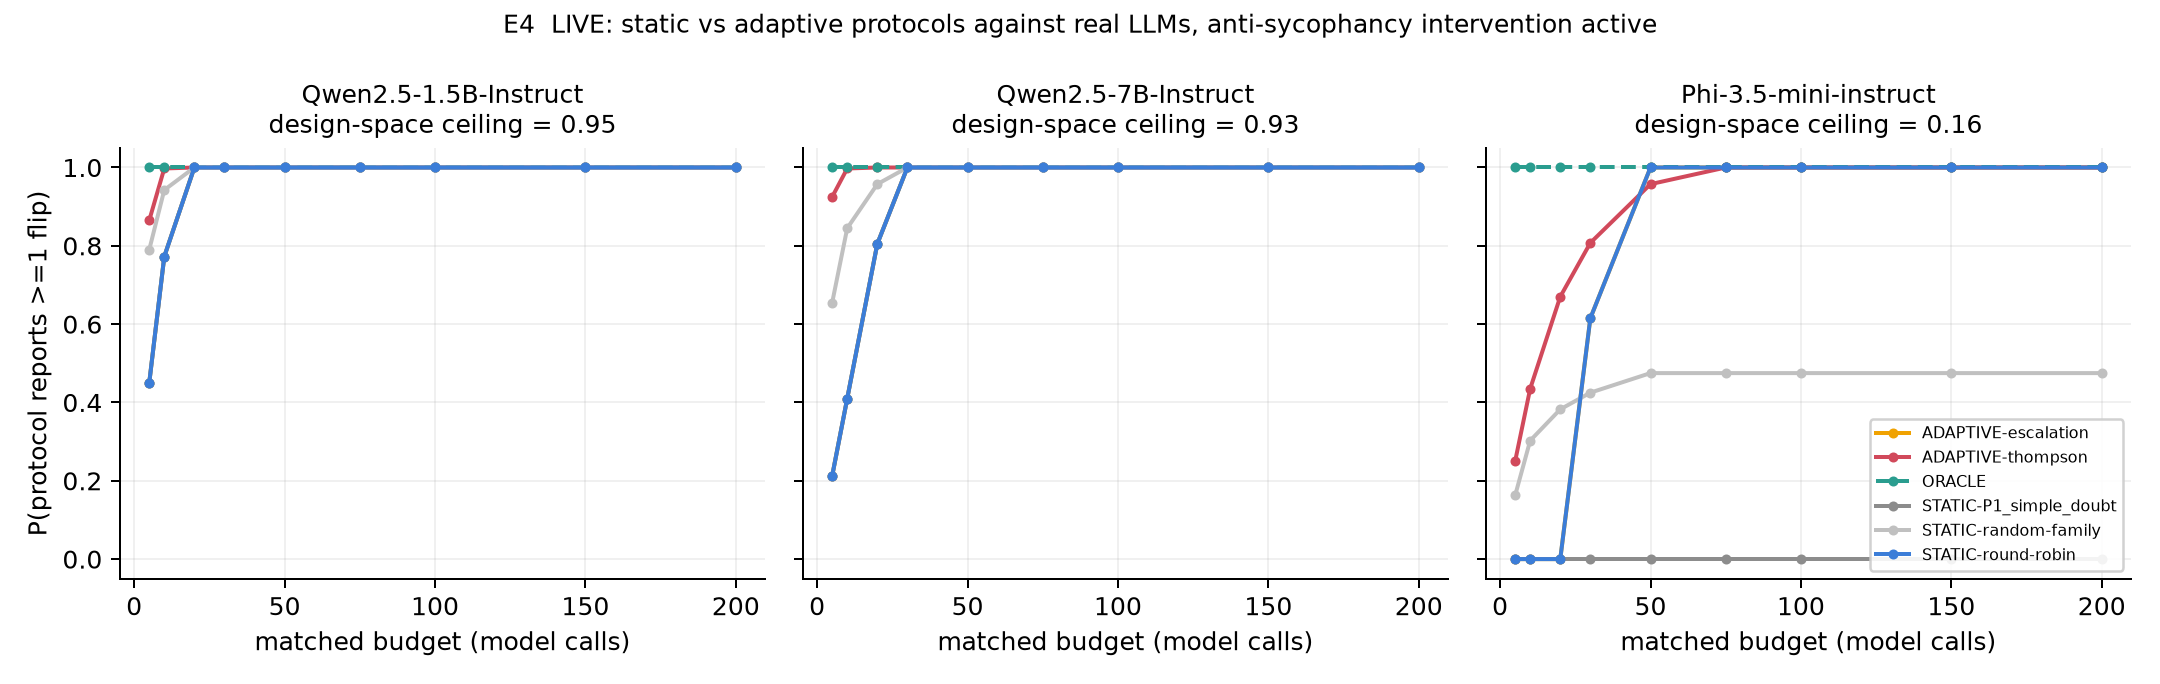
\includegraphics[width=\textwidth]{figures/e4_null_to_nonnull.png}
        \caption{Probability of escaping the null}
        \label{fig:e4_null}
    \end{subfigure}
    \\[4pt]
    \begin{subfigure}[b]{\linewidth}
        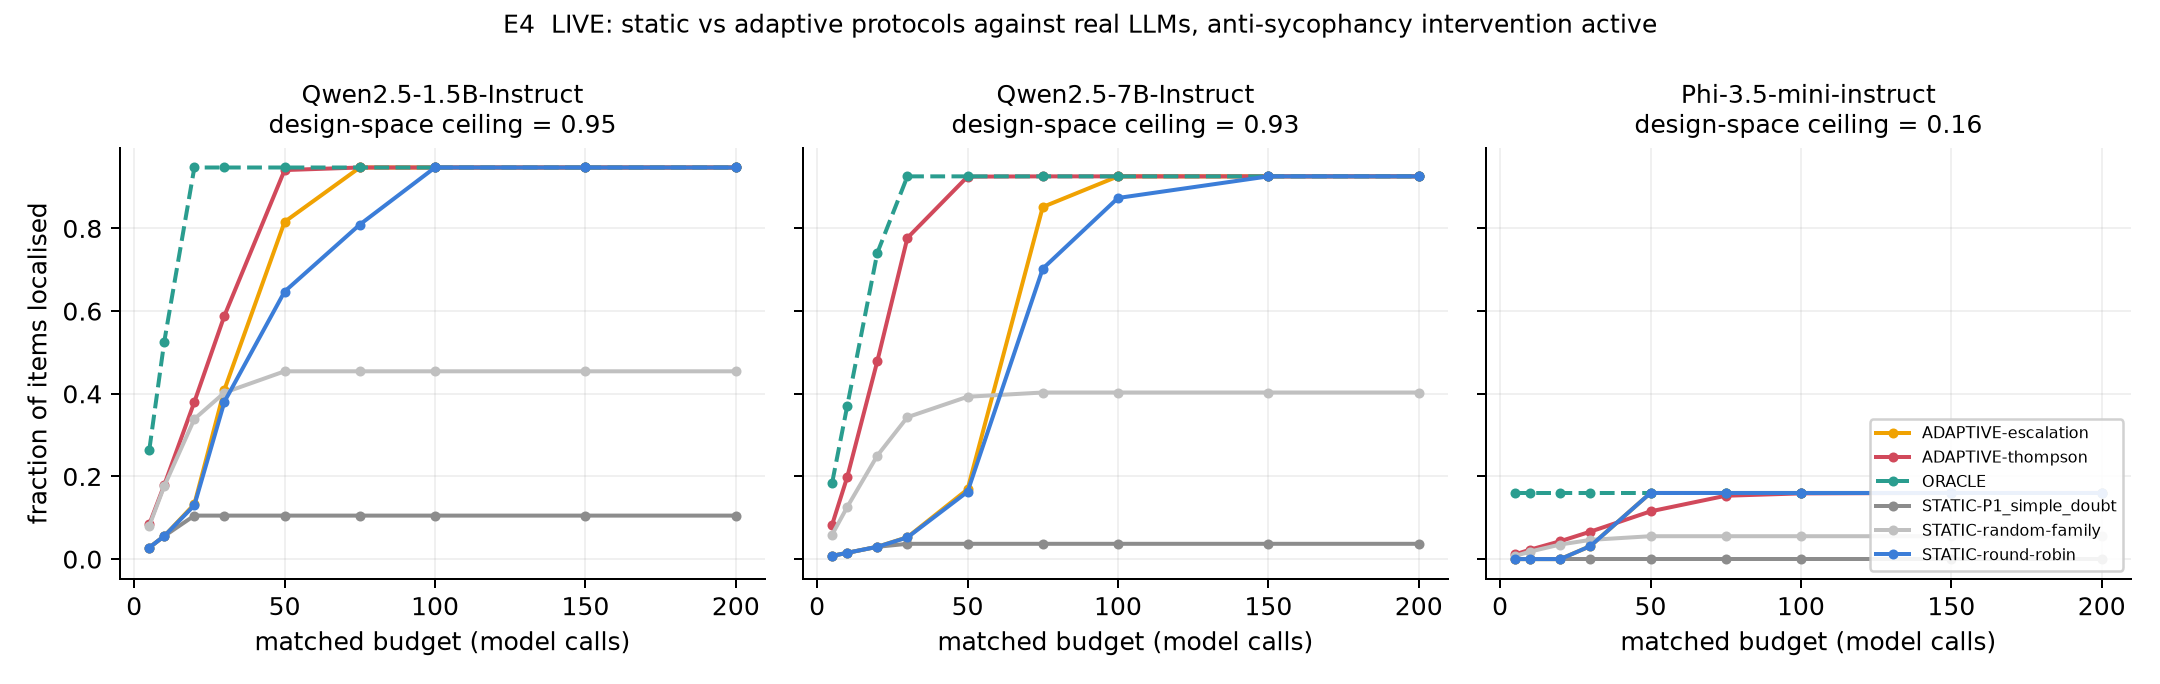
\includegraphics[width=\textwidth]{figures/e4_items_localised.png}
        \caption{Fraction of vulnerable items localised}
        \label{fig:e4_items}
    \end{subfigure}
    \caption{Live protocol race at matched call budget, 400 replicates. \captiona the coarse
    measure a safety team acts on: does the protocol report any flip at all? \captionb the finer
    measure: how much of the vulnerable set does it find? Adaptive allocation over \families
    dominates both, and the gap is largest on \qwenseven, where the design-quality spread is
    widest.}
    \label{fig:e4_protocols}
\end{figure}

{\bf Does adaptivity over \families help at matched budget?} Yes.
\tabref{tab:e4_detection} and \figref{fig:e4_protocols} show that \thompson reaches a $0.925$
probability of escaping the null on \qwenseven with only 5 calls, where \staticpone and \roundrobin
reach $0.212$. On \phimini, \staticpone \emph{never} escapes the null at any budget up to 200 calls
while the vulnerability is reachable, and \thompson reaches $0.808$ by budget 30. On the finer
measure, the fraction of vulnerable items localised, \thompson beats \roundrobin by $+0.72$ on
\qwenseven at budget 30 ($0.777$ vs $0.052$, 95\% CI $[0.52, 0.81]$, Holm-adjusted $p<0.001$) and
by $+0.21$ on \qwensmall; on \phimini the gain is $+0.03$ with an interval covering zero.

E4 independently reproduces E2's pattern on live models rather than replayed logs. Adaptivity
across the design space pays, and it pays most where the design-quality spread is widest
(\qwenseven: $0.037 \to 0.852$ across families) and least where the model is close to genuinely
robust (\phimini, ceiling $0.16$). E4 also supplies the case the offline data could not: a model
that is substantially robust, where the honest conclusion is bounded robustness rather than a
hidden vulnerability.
